\subsection{Attention-Based Architecture Comparison}

To further investigate the influence of attention mechanisms and transformer-based architectures on transfer learning performance, additional experiments are conducted using SE-enhanced ResNet-34 and ViT-Tiny. Both models are initialized with ImageNet pretrained weights and trained using the same hyperparameter configuration selected for the baseline ResNet-34 model.

To quantitatively compare different architectures, Table~\ref{tab:attention_comparison} summarizes the final validation accuracy of each model. Both the SE-enhanced ResNet-34 and ViT-Tiny achieve lower validation accuracy than the baseline ResNet-34, indicating that the additional attention mechanisms do not improve performance under the current experimental setting.

\begin{table}[H]
\centering
\caption{Validation accuracy comparison between different attention-based architectures.}
\label{tab:attention_comparison}
\begin{tabular}{l c}
\toprule
Architecture & Validation Accuracy \\
\midrule
Baseline ResNet-34 & 0.9538 \\
SE-enhanced ResNet-34 & 0.9443 \\
ViT-Tiny & 0.9348 \\
\bottomrule
\end{tabular}
\end{table}

\begin{figure}[h]
    \centering
    
    \begin{subfigure}{0.48\textwidth}
        \centering
        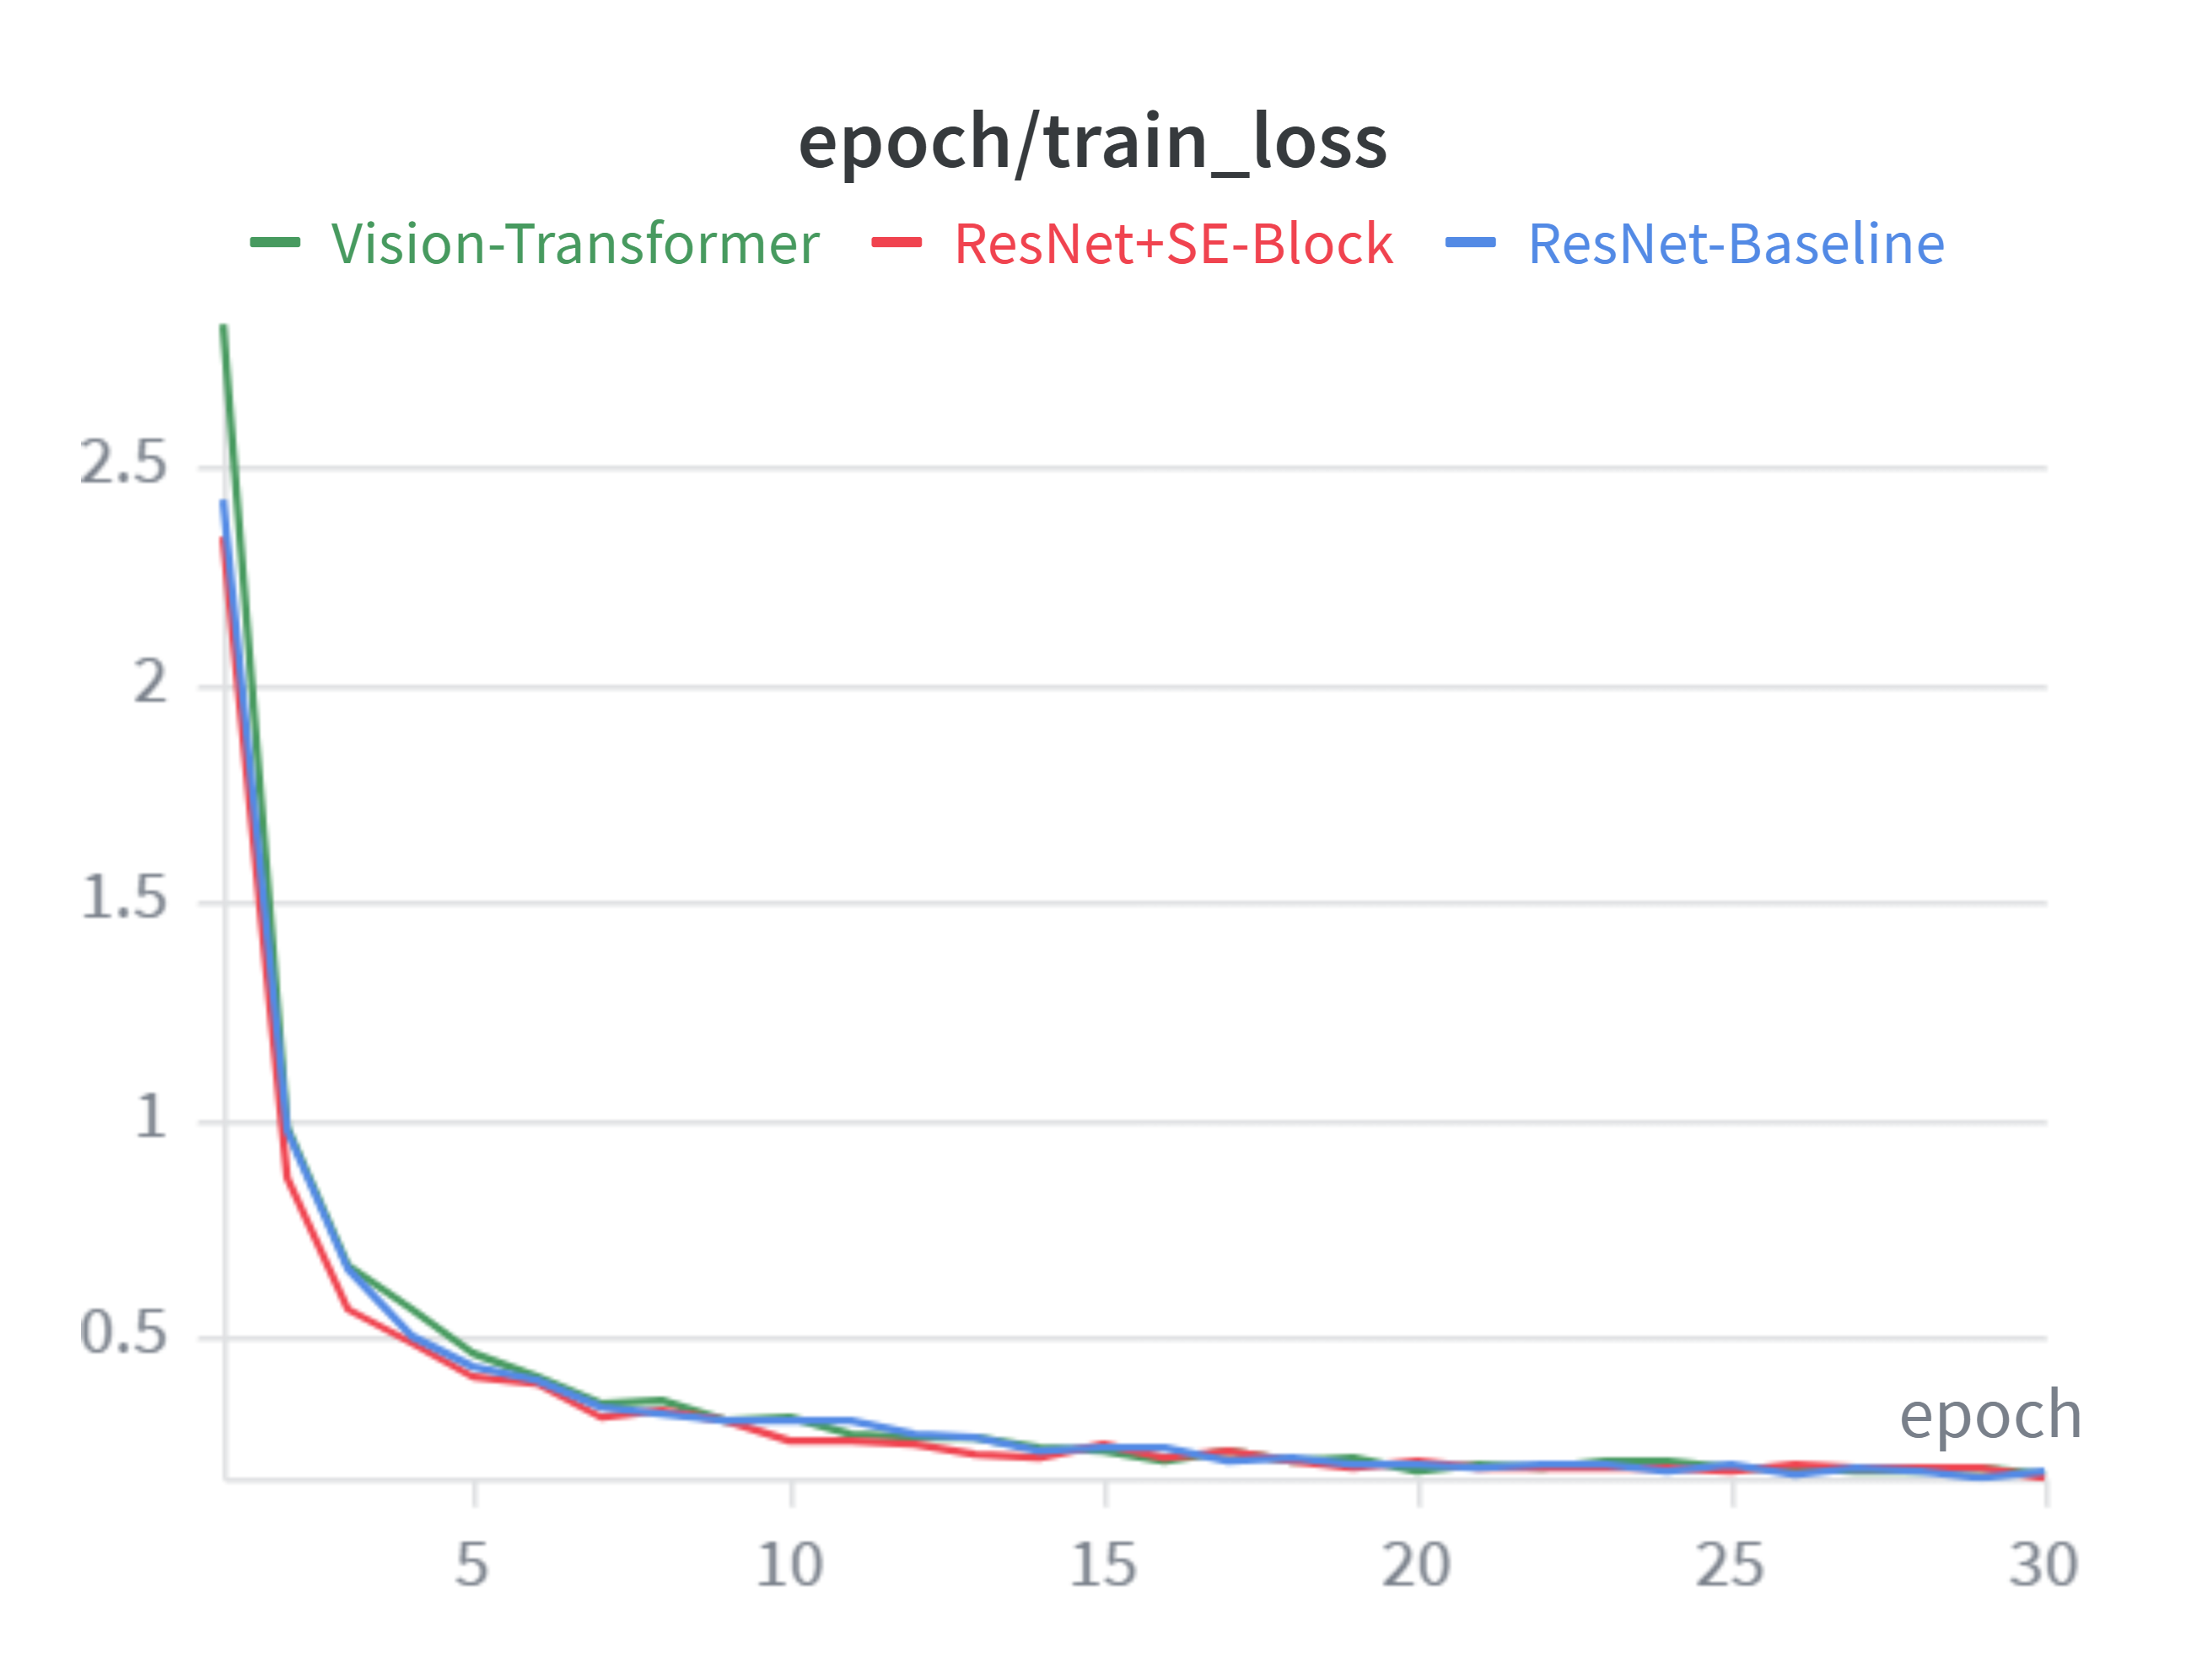
\includegraphics[width=\linewidth]{figures/task1/W&B Chart attention train loss.png}
        \caption{Training loss comparison.}
    \end{subfigure}
    \hfill
    \begin{subfigure}{0.48\textwidth}
        \centering
        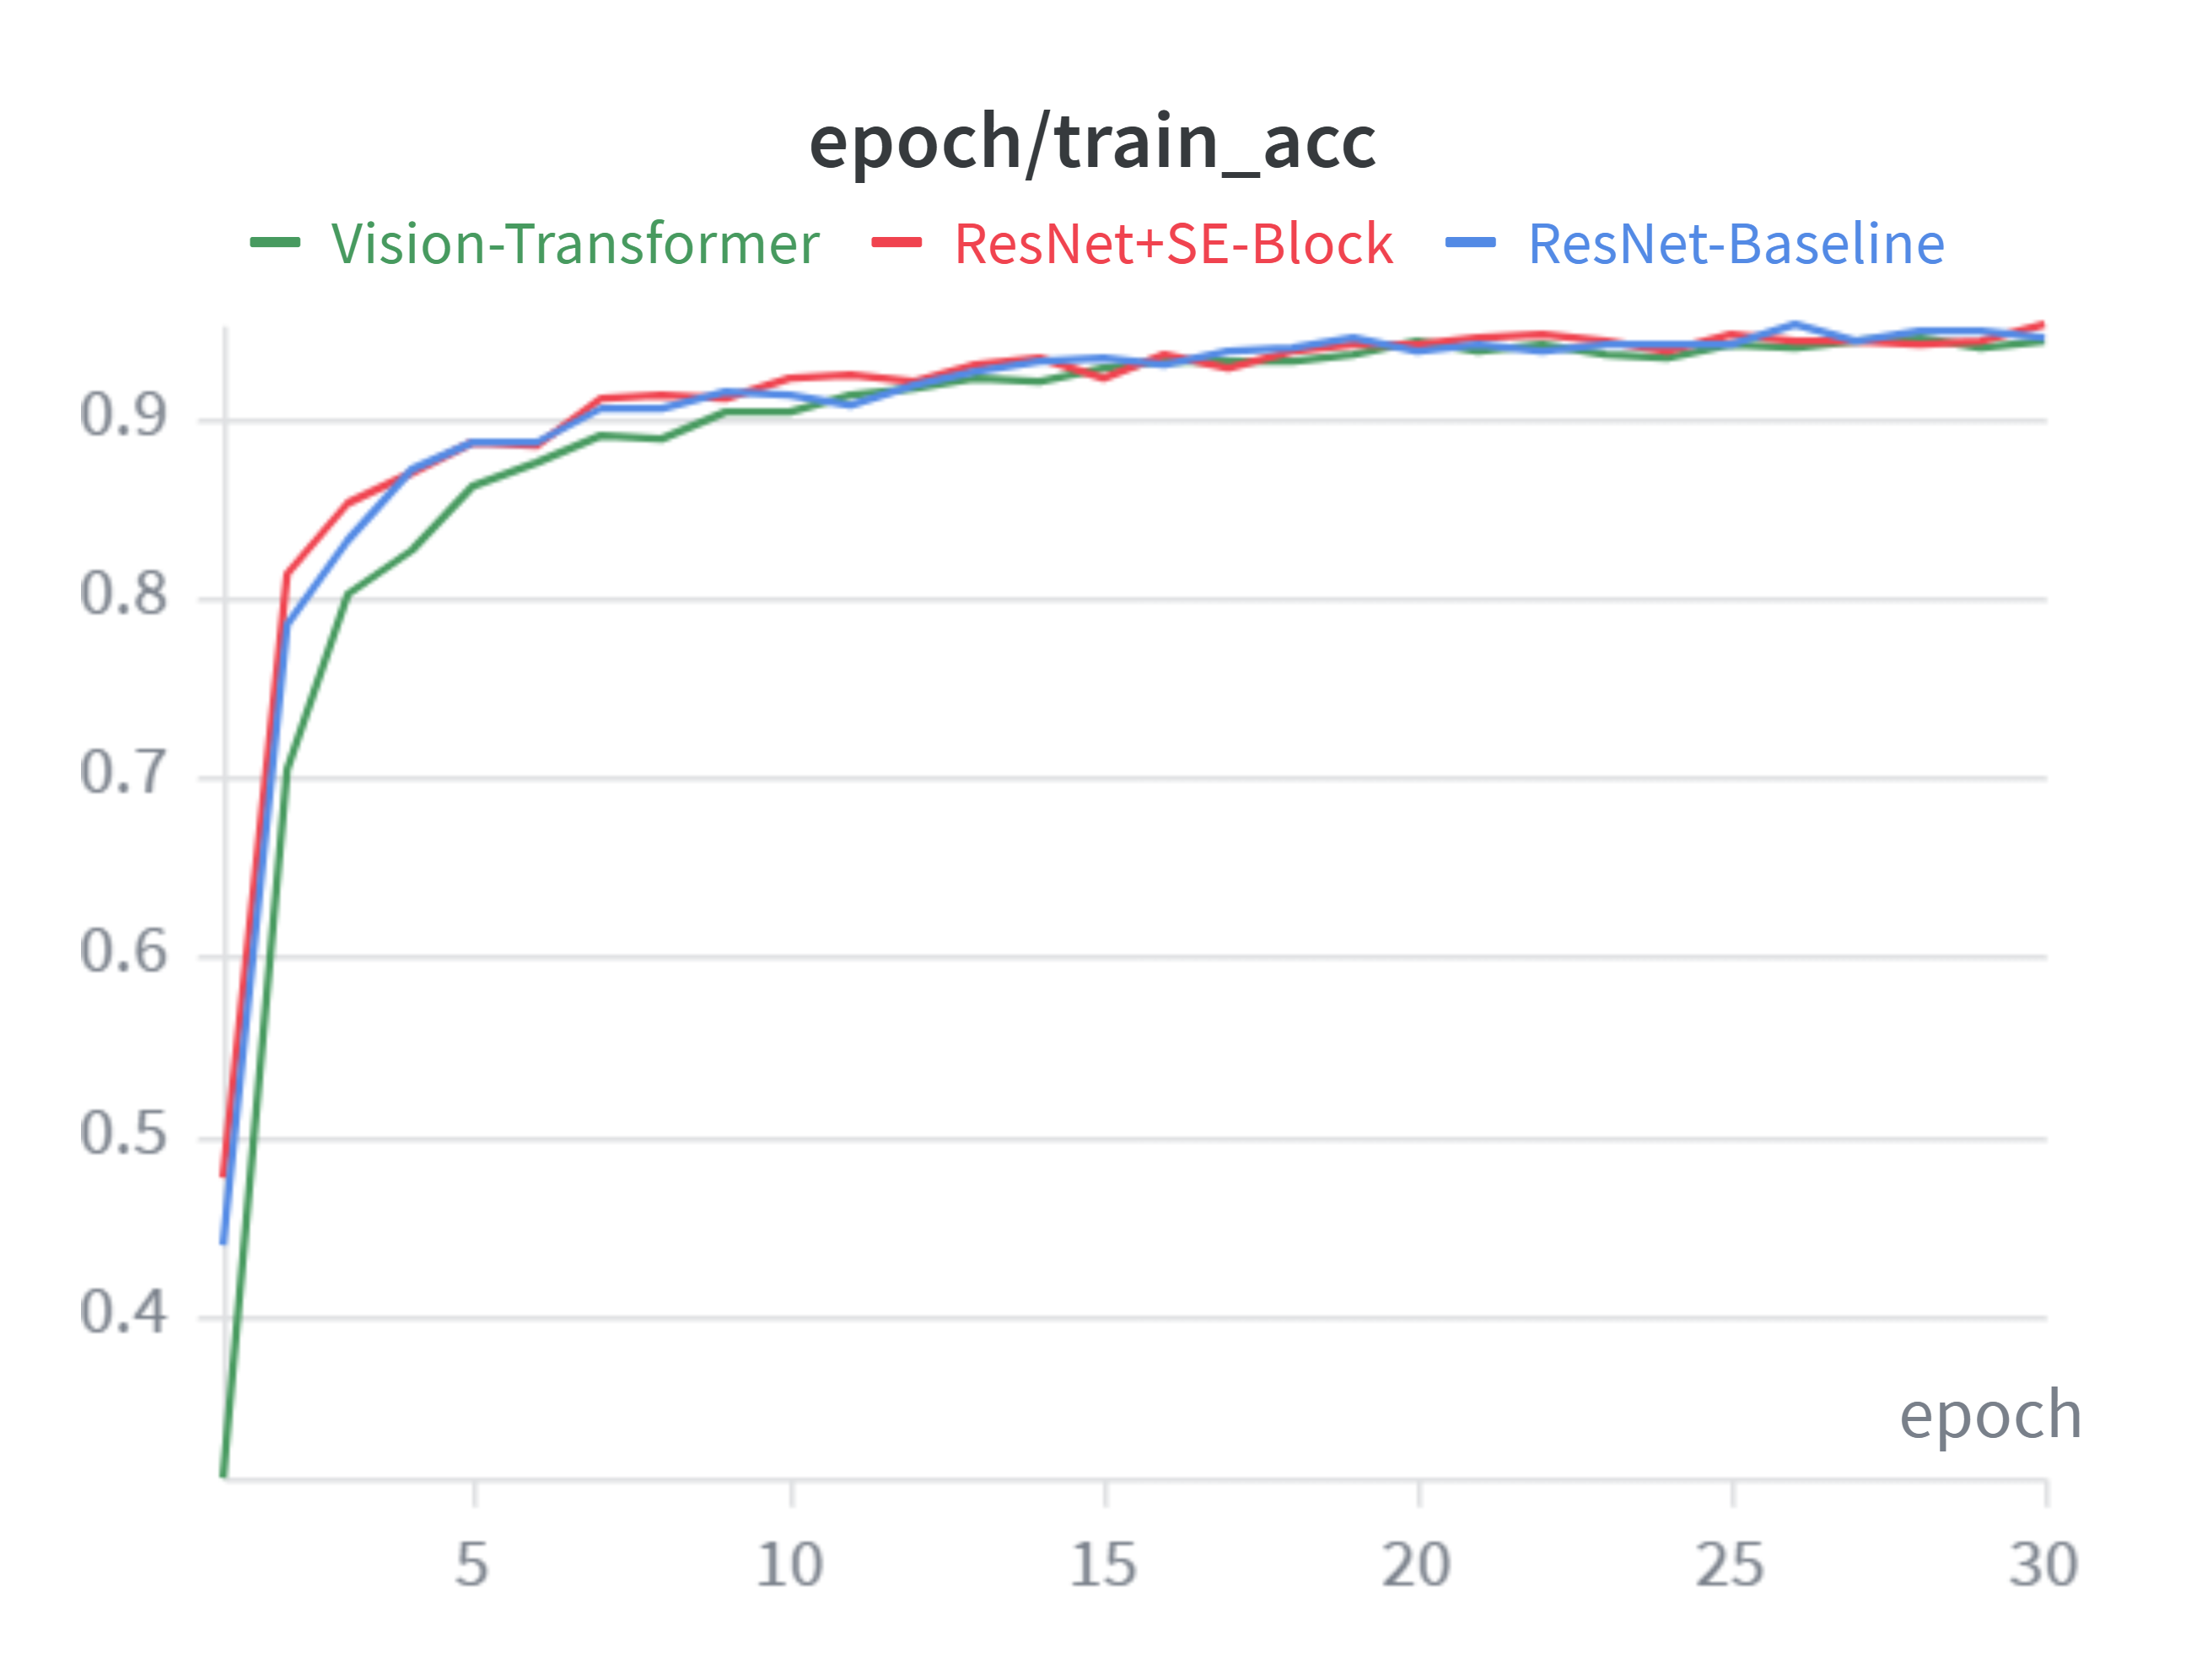
\includegraphics[width=\linewidth]{figures/task1/W&B Chart attention train acc.png}
        \caption{Training accuracy comparison.}
    \end{subfigure}

    \vspace{0.5em}

    \begin{subfigure}{0.48\textwidth}
        \centering
        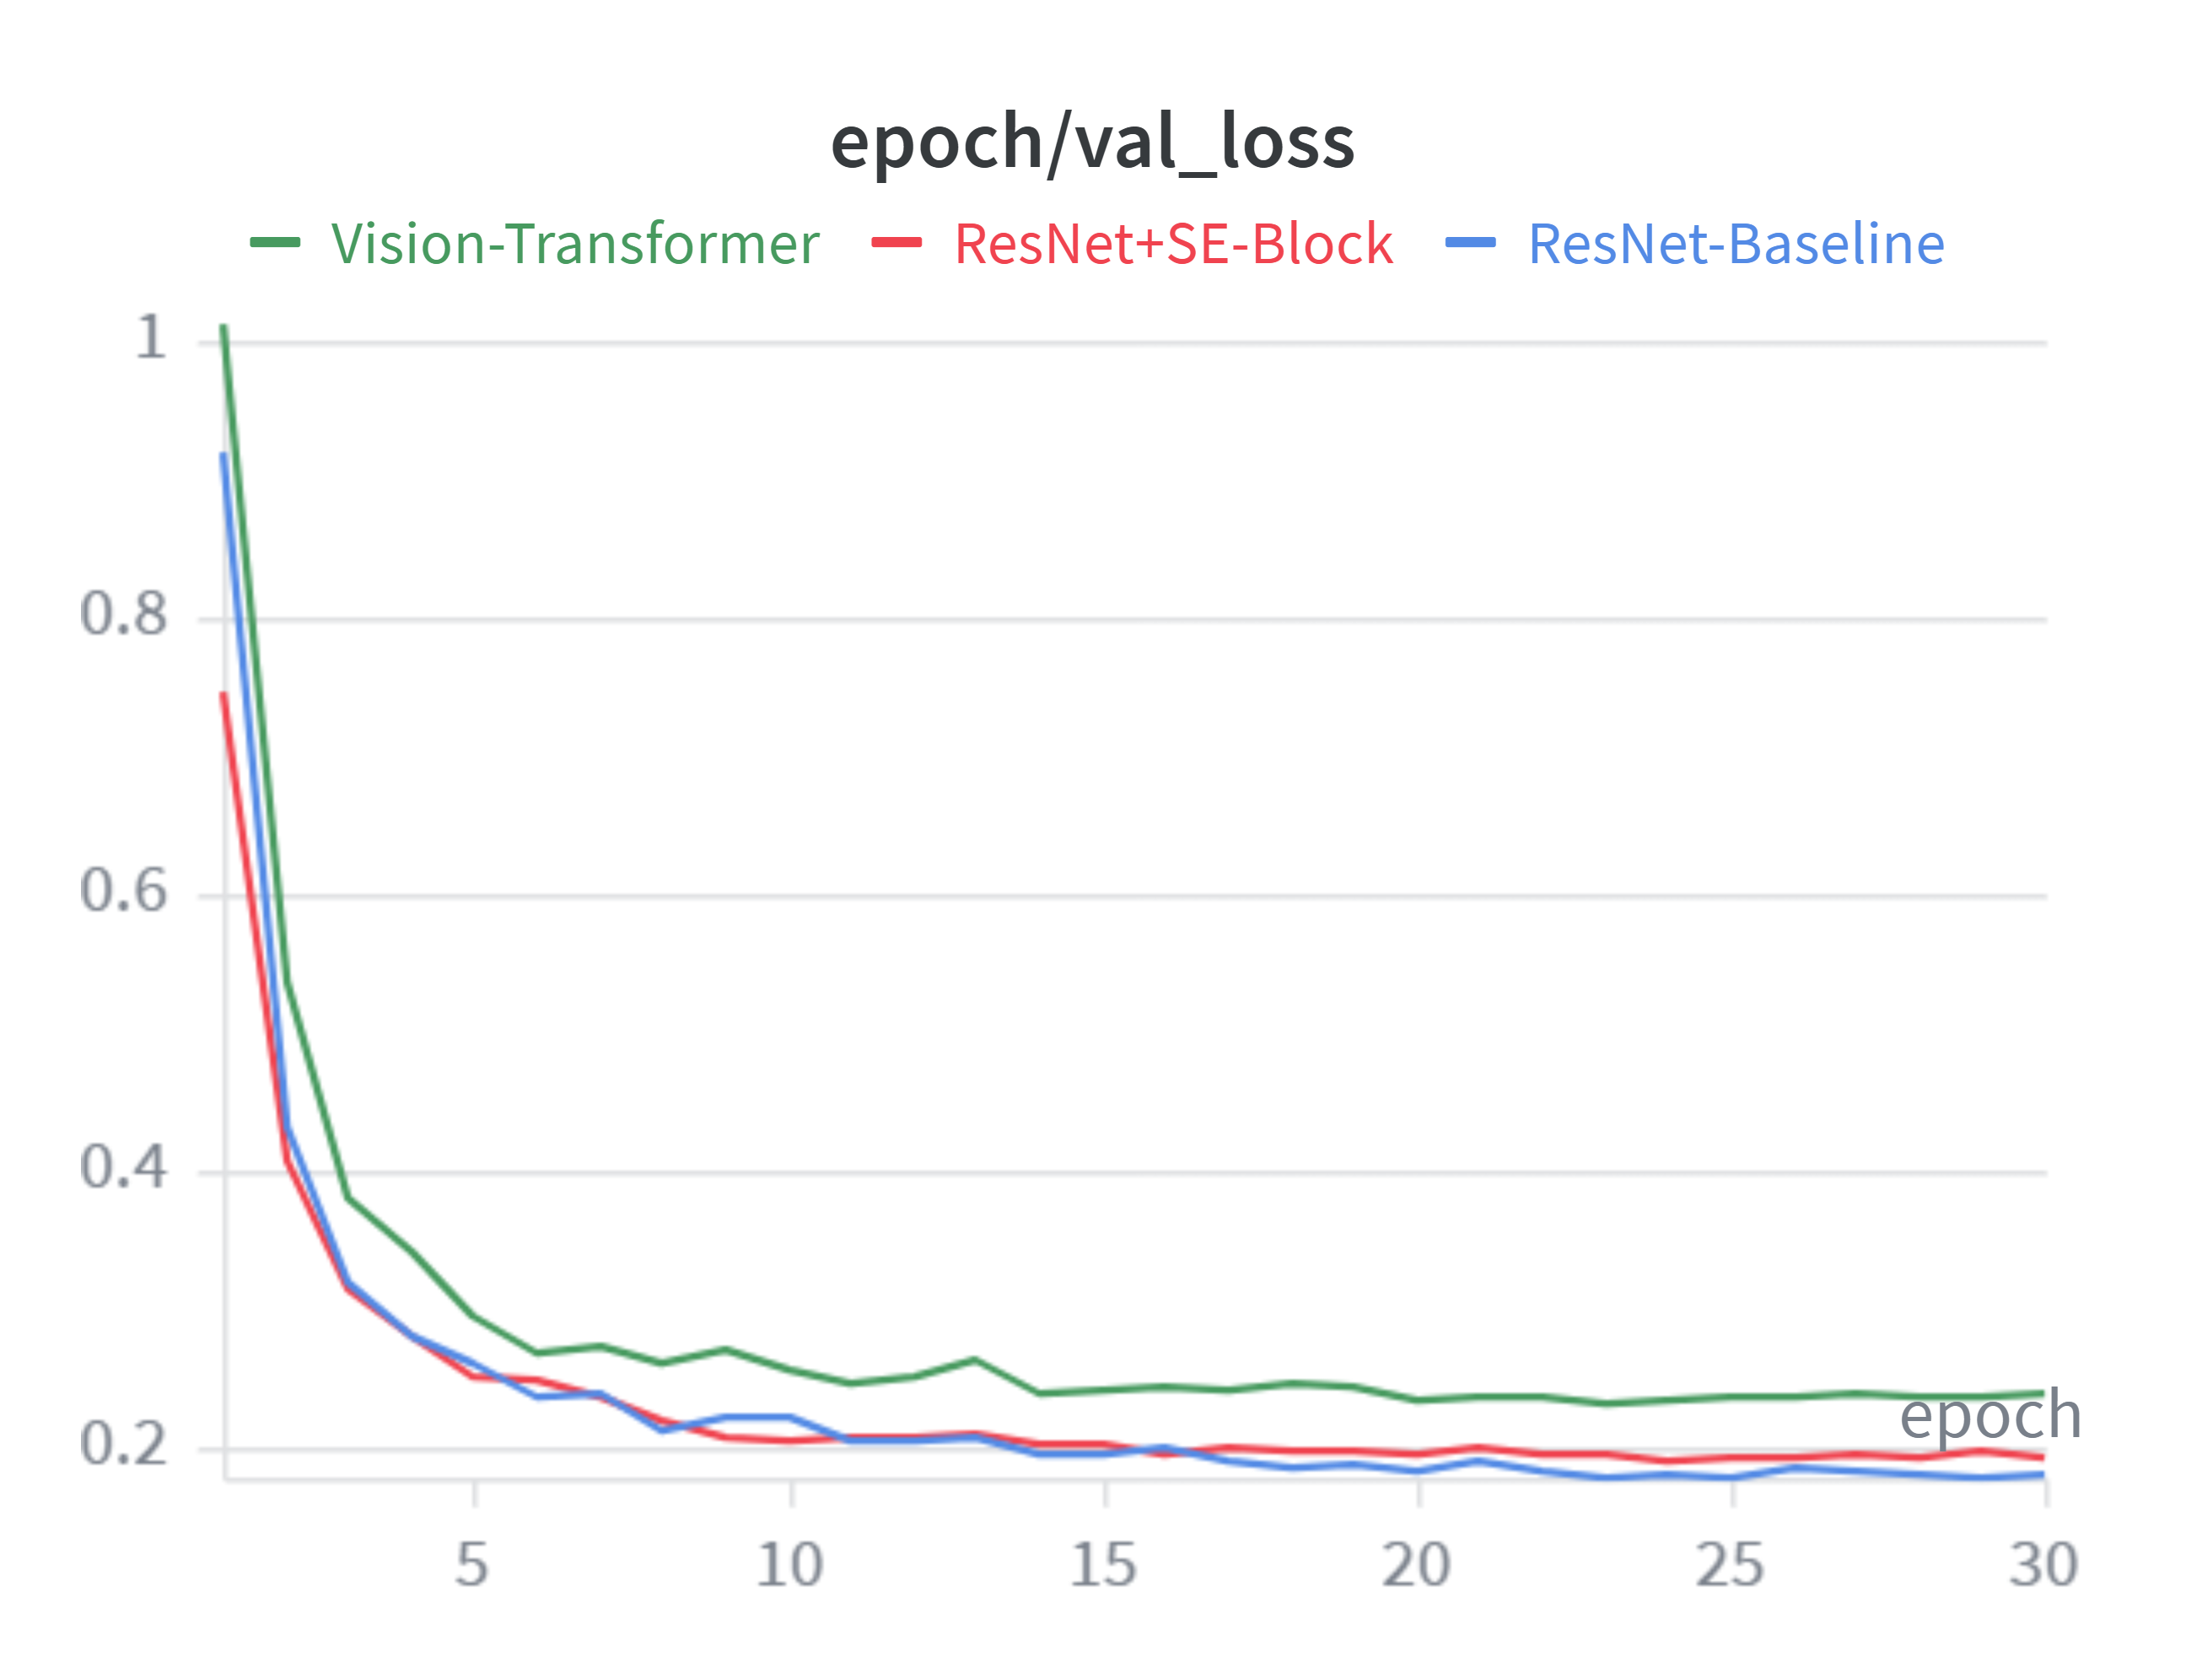
\includegraphics[width=\linewidth]{figures/task1/W&B Chart attention val loss.png}
        \caption{Validation loss comparison.}
    \end{subfigure}
    \hfill
    \begin{subfigure}{0.48\textwidth}
        \centering
        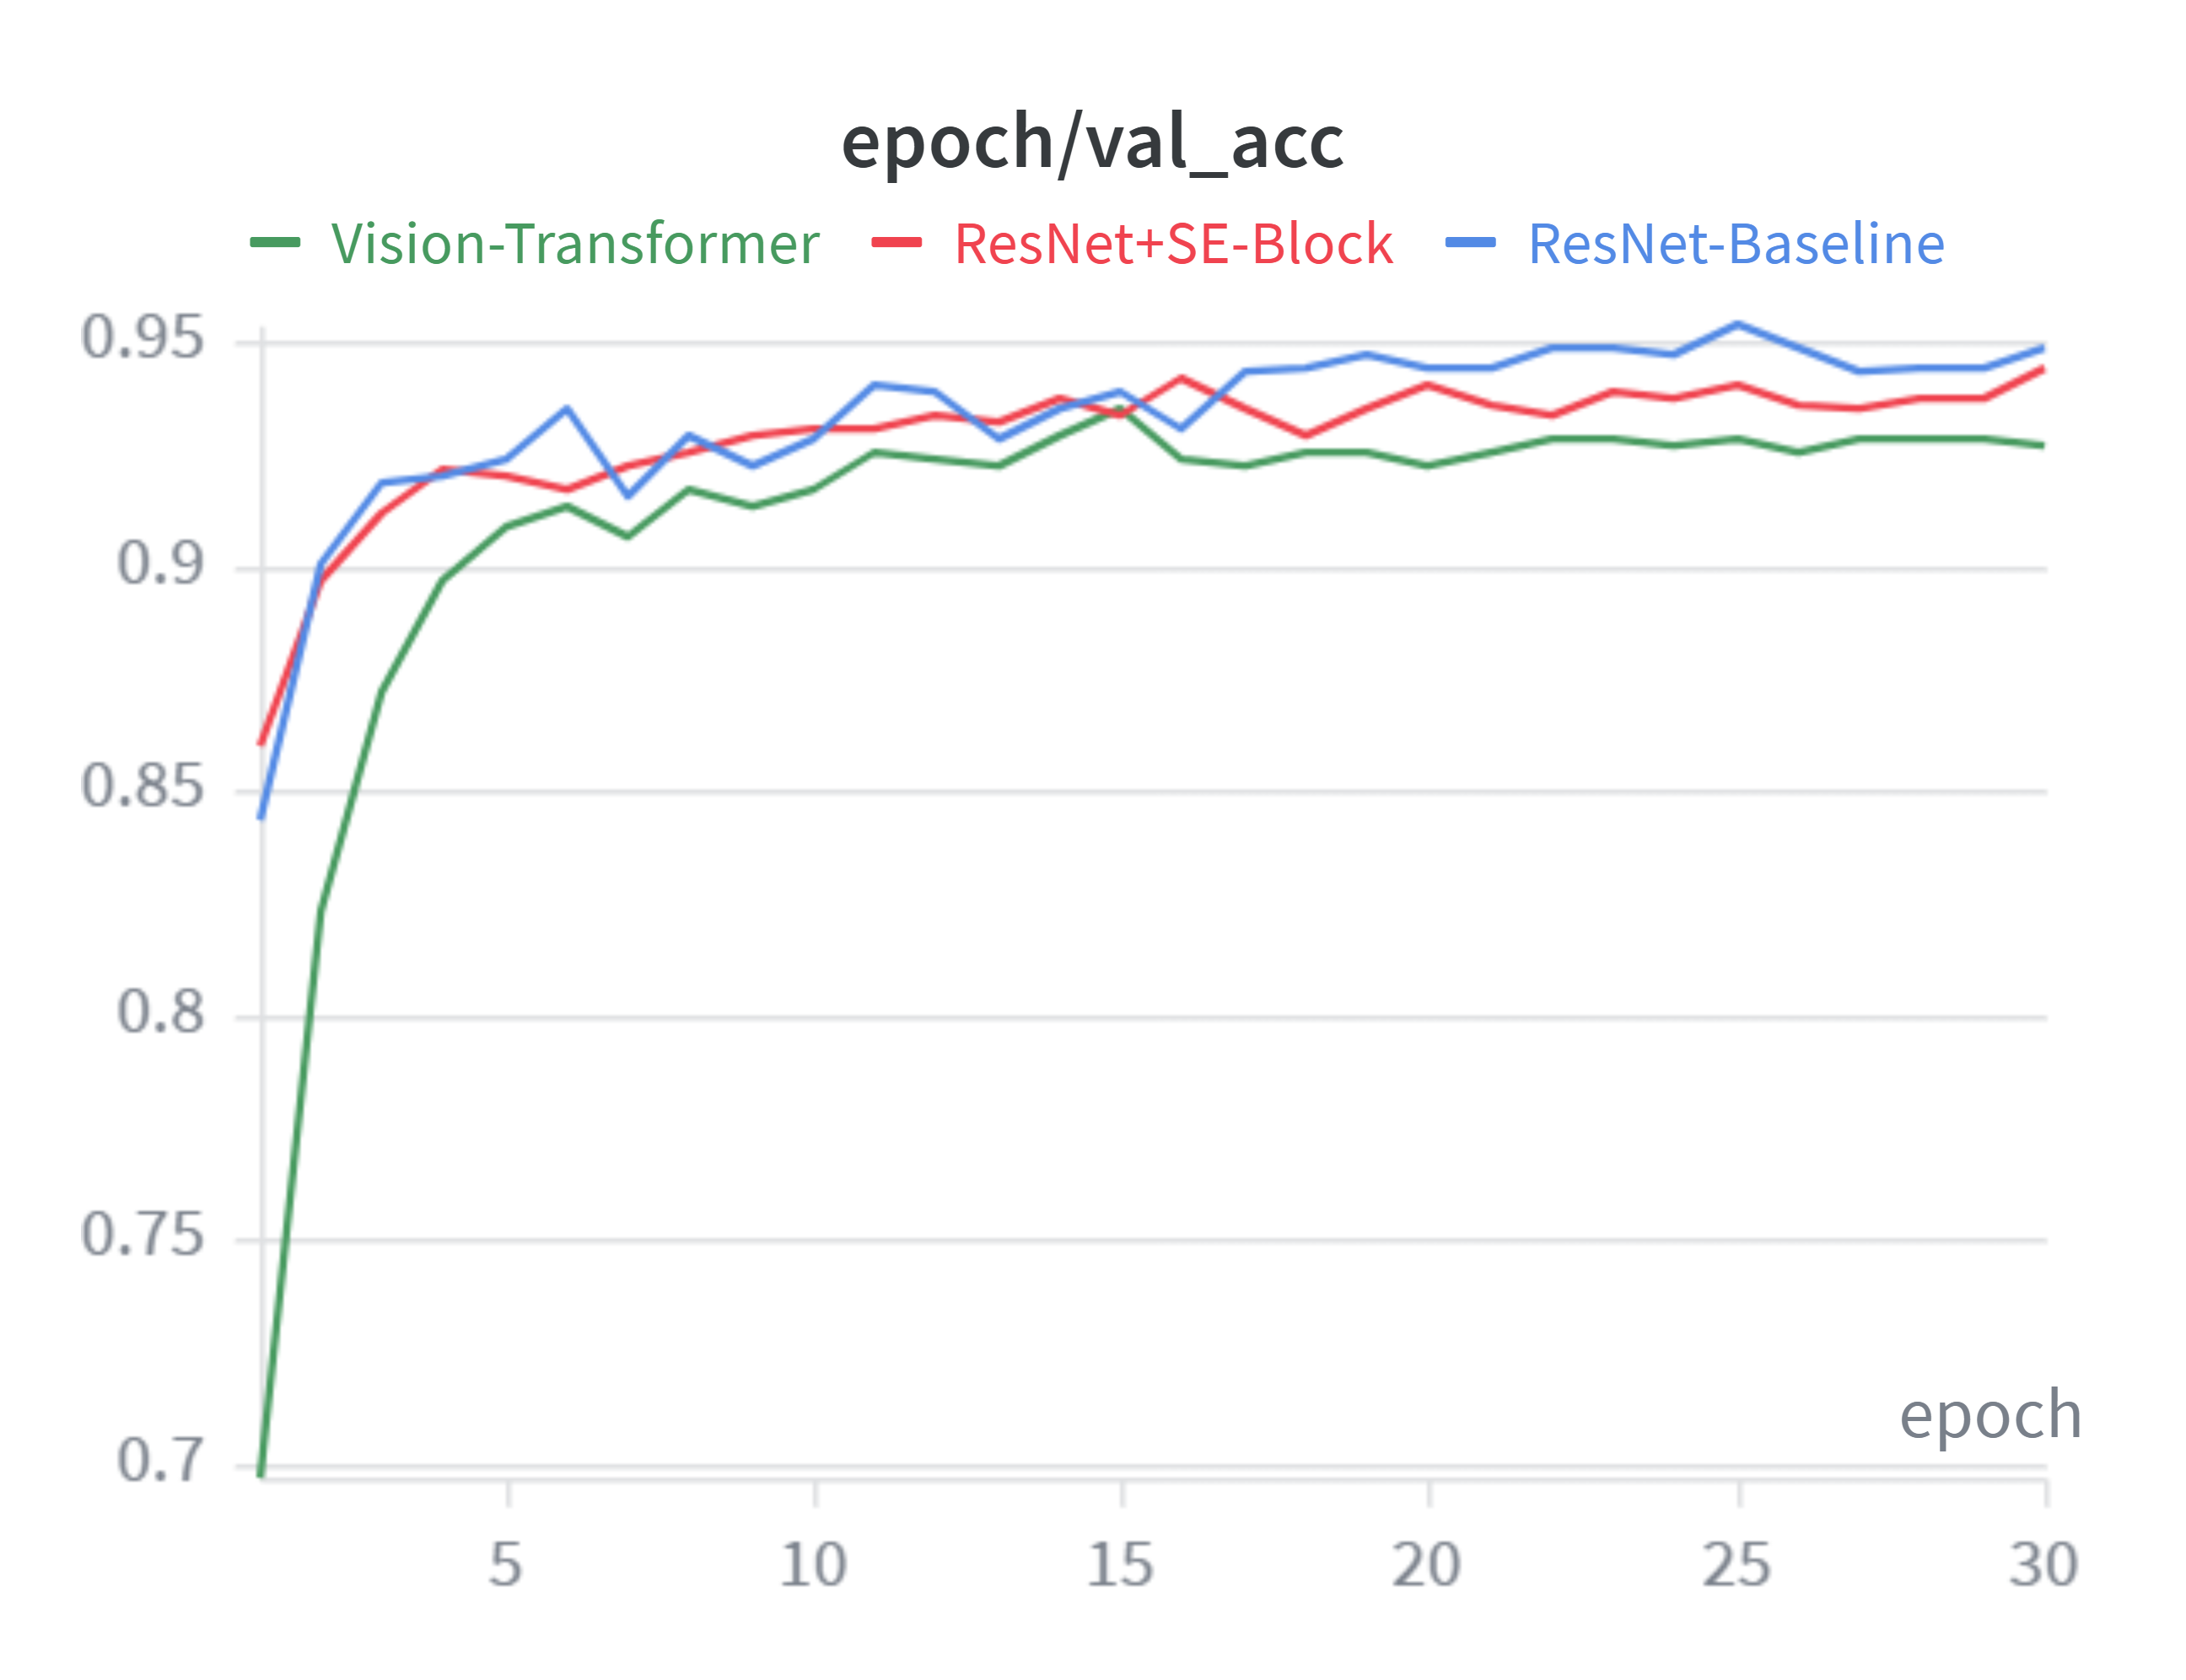
\includegraphics[width=\linewidth]{figures/task1/W&B Chart attention val acc.png}
        \caption{Validation accuracy comparison.}
    \end{subfigure}

    \caption{Comparison between baseline ResNet-34, SE-enhanced ResNet-34, and ViT-Tiny.}
    \label{fig:attention_comparison}
\end{figure}

As shown in Figure~\ref{fig:attention_comparison}(a) and Figure~\ref{fig:attention_comparison}(b), the three models exhibit highly similar optimization behavior on the training set. Their training losses decrease at comparable rates, and their training accuracies eventually converge to nearly the same level. ViT-Tiny shows slightly slower convergence during the early training stage, but the gap gradually diminishes.

More noticeable differences appear on the validation set. Figure~\ref{fig:attention_comparison}(c) and Figure~\ref{fig:attention_comparison}(d) show that the baseline ResNet-34 consistently achieves lower validation loss and higher validation accuracy than both SE-enhanced ResNet-34 and ViT-Tiny. The SE-enhanced model follows a validation trajectory very close to the baseline during early epochs, but eventually converges to slightly worse performance. ViT-Tiny exhibits consistently higher validation loss and lower validation accuracy throughout training.

One possible explanation is that the hyperparameter search process in Section~\ref{sec:hyperparameter_analysis} is performed specifically for the baseline ResNet-34 architecture. Since model selection is directly based on validation accuracy, the resulting hyperparameters are naturally biased toward the baseline model. In contrast, neither the SE-enhanced architecture nor ViT-Tiny receives architecture-specific hyperparameter tuning. Additional tuning strategies, such as attention-specific learning rate adjustment or longer training schedules, may therefore be necessary to fully exploit their capacity.

Another possible explanation is that the baseline transfer learning setting is already highly optimized for the Oxford-IIIT Pet dataset. With pretrained ImageNet features, carefully selected learning rates, and strong data augmentation, the baseline ResNet-34 already achieves validation accuracy above 95\%. Under this setting, introducing additional architectural complexity does not necessarily improve generalization performance.
